\section{Platforma Android}
Android to system operacyjny przeznaczony dla urządzeń mobilnych z jądrem Linuxa. Jego kolejne wersje zaczynają się na kolejne litery alfabetu i nawiązują do jakieś słodkiej przekąski lub deseru. Trzema najpopularniejszymi wersjami na rynku są Lollipop, Marshmallow i Nougat. Ostatnią wypuszczoną wersją jest Oreo (sytuacja z grudnia 2017). Każda z wersji udostępnia własny interfejs programowania aplikacji (ang. application programming interface) zwany \textbf{API}. Im nowsza wersja, tym wyższy jest poziom API, który daje nam szersze możliwości programistyczne.
\subsection{Programowanie obiektowe}
Podejście do sposobu programowania zmieniało się w czasie. Tradycyjnym podejściem było programowanie proceduralne. Polegało ono na rozdzieleniu danych od operujących na nich funkcji. Niestety takie podejście odizolowania danych od kodu może spowodować przypadkową ich modyfikację przez procedury, które nie były logicznie z nimi związane. Do takiego programu ciężko również było wprowadzić wszelkie modyfikacje. \par
Na początku lat 60. XX w. pojawiła się pierwotna koncepcja programowania obiektowego. Miała ona być bardziej naturalna dla ludzkiego mózgu, a samo programowanie stać się bardziej zgodne z rzeczywistością. Popularność zdobyła dopiero w okolicach lat 80. XX w., gdy pojawił się język C++ rozszerzający język C. Wyniknęło to ze wzrostu popularności graficznych interfejsów użytkownika, do których koncepcja programowania obiektowego sprawdza się wzorowo.\par Tworzenie programu zgodnego z koncepcją programowania obiektowego sprowadza się do rozdzielenia logiki na osobne klasy (typy danych), istniejące w tych klasach procedury oraz trzymaniu się konkretnych zasad. Te zasady nazywamy \textbf{paradygmatami programowania obiektowego}.
\paragraph{Abstrakcja (ang. abstraction)}\mbox{}\\ Sprowadzenie danego problemu do prostszej postaci. Polega na wyznaczeniu dla obiektów cech, niezbędnych dla algorytmów, ale jednocześnie niezależnych od implementacji.
\paragraph{Enkapsulacja (ang. encapsulation)}\mbox{}\\ Ukrycie cech obiektu. Zewnętrzne otoczenie nie może zmienić danych znajdujących się wewnątrz obiektu w nieoczekiwany sposób. Każda klasa udostępnia abstrakcyjną reprezentację siebie zwaną interfejsem. Za jego pomocą zewnętrzne otoczenie może się komunikować z danym obiektem.
\paragraph{Polimorfizm (ang. polymorphism)}\mbox{}\\ Używanie wartości zmiennych i podprogramów na kilka różnych sposobów. Wykazywanie przez metodę różnych form działania w zależności od tego jaki typ obiektu jest wskazywany przez wskaźnik lub referencję.
\paragraph{Dziedziczenie (ang. inheritance)}\mbox{}\\ Porządkuje polimorfizm i enkapsulację przez definiowanie i tworzenie specjalizowanych obiektów na podstawie bardziej ogólnych.

\paragraph{Obiekt a klasa}\mbox{}\\
Podstawową cegiełką każdego programu zgodnego z koncepcją programowania obiektowego jest obiekt. Obiekt to nie to samo co klasa. Klasa opisuje pola (zmienne) i metody (procedury) dla wszystkich reprezentantów tej klasy, czyli obiektów.\par Zarówno pola jak i metody muszą mieć określony poziom dostępu. Wyróżniamy trzy poziomy dostępu: publiczny, chroniony oraz prywatny. Dostęp publiczny oznacza, że dany atrybut może zostać użyty zarówno w obiekcie tej klasy jak i poza nim. Dostęp chroniony pozwala na używanie atrybutów tylko w obiekcie tej klasy, ale również w obiektach dziedziczących z tej klasy. Dostęp prywatny nie zezwala na używanie atrybutów klasy żadnym obiektom nie będącymi reprezentacją tej klasy. Jeśli nie podamy jawnie poziomu dostępu do danego atrybutu, zostanie on potraktowany jako prywatny, jest to domyślny poziom dostępu.\par Wszystkie pola klasy powinny mieć dostęp prywatny, a modyfikację tych pól powinny być ewentualnie możliwe przez publiczne metody wykonujące operacje na tych polach. Metodę publiczną pobierająca wartość danego pola nazywamy getter'em, natomiast metodę ustawiającą wartość danemu polu setter'em.\par Każdy z atrybutów może być dodatkowo statyczne dla danej klasy. Oznacza to, że możemy odwołać się do tego atrybutu bez tworzenia reprezentanta tej klasy. Najczęściej takie statyczne atrybuty mają dostęp publiczny. Jeśli metoda nie jest zadeklarowana jako statyczna, może zostać zadeklarowana jako wirtualna. Oznacza to, że nie można wywołać tej metody dopóki nie zostanie ona nadpisana w klasie dziedziczącej.\par Klasa implementuje tylko abstrakcyjny typ danych więc pamięć przydzielana jest dopiero do obiektów, a nie do samej klasy. Natomiast obiekt jest już strukturą zawierającą dane oraz funkcje pracujące na tych danych. Każdy obiekt będący reprezentantem danej klasy nazywamy instancją tej klasy. Każda instancja ma taki sam zestaw pól oraz metod, jednakże mogą się różnić wartościami pól wewnątrz. Tworzenie instancji następuje przez wywołanie konstruktora. Konstruktor to specjalna metoda w klasie, musi mieć ona identyczną nazwę co klasa. Po wywołaniu konstruktora następuje alokacja pamięci dla obiektu, połączenie tego obszaru z metadanymi z klasy, wykonaniu kodu klasy bazowej oraz konstruktora. Dopiero wtedy nasz obiekt zaczyna fizycznie istnieć. Jednakże zmienna obiektowa nie przechowuje wewnątrz siebie danych obiektu, ona przechowuje referencję do tego obiektu. Referencja to wartość, która informuje o lokalizacji danych obiektu w pamięci.\par Istnieją klasy, których instancji nie można utworzyć. Nazywamy je klasami abstrakcyjnymi. Klasa abstrakcyjna musi posiadać conajmniej jedną metodę wirtualną w sobie. Jeśli posiada wyłącznie metody wirtualne, jest wówczas nazywana interfejsem klasy.


\subsection{Programowanie na Androida}
Android nie ma ściśle określonej technologii, za pomocą której można tworzyć dla niego aplikacje. Wybór zależy od efektów jakie chcemy osiągnąć. Technologii za pomocą, których chcielibyśmy tworzyć aplikację jest bardzo dużo, jednakże można je podzielić na dwa rodzaje. Programowanie natywne (np. Android oraz JNI) zwięszy wydajność aplikacji. Programowanie multiplatformowe (np. Apache Cordova oraz Xamarin) zwiększy przenośność. 
\paragraph{Android-Java}\mbox{}\\
Jest najpopularniejszą technologią do tworzenia aplikacji na Androida. Jak nazwa wskazuje, bazuje ona na języku Java, chociaż często nazywa się tę technologię po prostu Android. Programista ma dostęp do obszernej dokumentacji całego języka.
\paragraph{Java Native Interface (JNI)}\mbox{}\\
Java Native Interface jest to framework, który umożliwia aplikacji Java uruchomionej na wirtualnej maszynie Javy (ang. Java Virtual Machine) wołać funkcje natywne. To znaczy takie, które wykonują się bezpośrednio na komponentach komputera, napisane w innych językach programowania takich jak C czy C++. Możliwe jest także wołanie metod kodu Java przez natywne aplikacje. Możliwe jest użycie tego interfejsu na platformie Android. Kod natyny wykonuje się znacznie szybciej w porównaniu do Javy. Kolejną powodem do stosowania JNI jest fakt, że istnieje wiele bibliotek i narzędzi w językach C i C++, które nie mają swoich odpowiedników dla języka Java. Wywołanie metody natywnej z poziomu kodu Javy jest kosztowne. Pojedyncze wywołanie takiej metody trwa znacznie dłużej niż zawołanie takiej metody w obrebie jednej platformy. Dodatkowo tablice często są kopiowane dla funkcji natywnej, a po jej wykonaniu kopiowane są z powrotem dla kodu Java. Przykładowy kod z wykorzystaniem JNI w środowisku Android, zwracający łańcuch znaków: 
\begin{lstlisting}[language=C]
#include <jni.h>
#include <string>

extern "C"
JNIEXPORT jstring JNICALL
Java_com_example_maciej_myapplication_MainActivity_stringFromJNI(
        JNIEnv *env,
        jobject /* this */) {
    std::string hello = "Hello from C++";
    return env->NewStringUTF(hello.c_str());
}
\end{lstlisting}

Dodatkowo w kodzie Java potrzebna jest deklaracja funkcji
\begin{lstlisting}[language=C]
public native String stringFromJNI();
\end{lstlisting}
\paragraph{Apache Cordova}\mbox{}\\
Cordova to framework, który opakowuje aplikację HTML/JavaScript do macierzystego kontenera, który ma dostęp do funkcji urządzenia na kilku platformach. Funkcje te są udostępniane za pośrednictwem zunifikowanego interfejsu JavaScript API, dzięki czemu można łatwo napisać jeden zestaw kodu.
\paragraph{Xamarin}\mbox{}\\
Xamarin jest platformą, na której w język C\# jesteśmy w stanie stworzyć aplikacje na Androida, WindowsPhona i iOS jednocześnie. Posiada specjalne zestawy narzędzi dla programistów (ang. software development kit) zwane SDK: Xamarin.iOS i Xamarin.Android. Tworzenie na WindowsPhona nie wymaga dodatkowego SDK.
\subsection{Intencja}
\textbf{Intencja (ang. Intent)} to abstrakcyjny opis akcji jaką chcemy wykonać. Możliwości wykonania akcji przy pomocy Intencji jest bardzo dużo. Do podstawowych zalicza się przejście do kolejnego widoku w aplikacji czy wykonanie zdjęcia. Pełni ona rolę spoiwa między kodem różnych aplikacji. Opisuje ona czynność do wykonania, dzięki czemu osobna aplikacja realizuje swoją pracę i odsyła ewentualne wyniki. Pierwszorzędnymi atrybutami struktury Intencji jest opis akcji do wykonania oraz ewentualne dane niezbędne do wykonania tej akcji. Do drugorzędnych atrybutów należą:
\begin{itemize}
\item Kategoria (ang. category) - zapewnia dodatkową informację na temat akcji do wykonania.
\item Typ (ang. type) - precyzuje typ danych jaki jest przekazywany.
\item Komponent (ang. component) - precyzuje nazwę komponentu (klasy), która będzie używała Intencji. Zazwyczaj jest to określone z pozostałych atrybutów i na podstawie tego dopasowywany jest komponent, który obsłuży daną akcję. Ustalenie tego atrybutu powoduje, że pozostałe są opcjonalne.
\item Dodatki (ang. extras) - przechowuje wszelkie dodatkowe informacje jakie chcielibyśmy przekazać do komponentu.
\end{itemize}
Ponadto każdej Intencji możemy ustawić flagi. Lista dostępnych flag jest opisana w dokumentacji Androida. Zapewniają one dodatkowe informacje konfiguracyjne np. ustawienie flagi \textit{FLAG\_FROM\_BACKGROUND} informuje, że dana Intencja pochodzi od procesu w tle, a nie od interakcji użytkownika.
Istnieją dwie podstawowe formy Intencji:
\begin{itemize}
    \item Jawne (ang. explicit) Intencje mają określony atrybut komponent. Można tego dokonać poprzez metodę \textit{setComponent()} lub \textit{setClass()}. Dzięki temu, jednoznacznie jest ustalona klasa, która ma zająć się wykonaniem akcji określonej w Intencji.
    \item Niejawne (ang. implicit) Intencje nie określają atrybutu komponent. Muszą natomiast, poprzez pozostałe atrybuty, zawierać wystarczająco dużo informacji, aby system określił, który z dostępnych komponentów będzie najlepszy do przeprowadzenia danej akcji.
\end{itemize}
Rozstrzygnięcie niejawnej Intencji następuje na podstawie trzech atrybutów: akcji, typu i kategorii. Korzystając z tych informacji wykonywane jest zapytanie w menadżerze pakietów dla komponentu, który może obsłużyć Intencję. Decyzję o tym czy dany komponent zostanie użyty określa się w następujący sposób. Jeśli został ustalony atrybut akcja i/lub typ w Intencji, to musi on być również wymieniony przez komponent jako obsługiwany.  Natomiast określenie kategorii odnosi się do Aktywności, musi ona obsługiwać daną kategorię, aby zrealizować Intecję.\cite{intent}
\subsection{Manifest}
Każda aplikacja w technlogii Android musi posiadać plik AndroidManifest.xml w swoim głównym folderze. Zapewnia nazwę pakietu Java dla aplikacji, która pełni rolę unikalnego identyfikatora. Manifest dostarcza podstawowych informacji o aplikacji (etykieta, ikona) do systemu Android, które musi posiadać, zanim będzie mógł uruchomić kod aplikacji.  Zawiera listę bibliotek, z którymi aplikacja musi być połączona. Opisuje komponenty aplikacji oraz podaje nazwy klas ich implementujących. Deklaruje minimalny poziom interfejsu API Androida oraz uprawnienia, które muszą być spełnione do prawidłowego funkcjonowania. Zgoda użytkownika co do uprawnień jest niezbędna, aby aplikacja mogła korzystać z chronionych części API. Niezbędnym elementem do ustawienia jest ustalenie widoku, który się wyświetli przy pierwszym uruchomieniu. Dokonuje się tego poprzez Filtr Intencji (ang. Intent Filter). Wystarczy w elemencie opisującym Aktywność wstawić Filtr Intencji z odpowiednimi wartościami atrybutów akcji oraz kategorii (odpowiednio \textit{android.intent.action.MAIN} oraz \textit{android.intent.category.LAUNCHER}).\cite{manifest}
\subsection{Zasoby}
W dzisiejszych czasach często wprowadza się zmiany w istniejących aplikacjach. Może to być spowodowane zmianą właściciela aplikacji, decyzją ulepszenia aplikacji lub po prostu ludzkim kaprysem. Dlatego wysoki nacisk kładzie się na to, aby aplikacja była łatwo modyfikowalna. Android zapewnia mechanizm określonym jako \textbf{Zasoby (ang. Resources)}.\par Wszelkie Zasoby powinny zostać podzielone i umieszczone w specjalnych podfolderach katalogu z zasobami o nazwie \textit{/res}. Mamy kilka takich specjalnych podfolderów do wyboru, między innymi folder \textit{/drawable} służy do przechowywania w nim obrazków wyświetlanych w aplikacji. Folder \textit{/color} zawiera zdefiniowane kolory używane w aplikacji. Folder \textit{/layout} zawiera pliki xml opisujące widoki używane w komponentach graficznych aplikacji. Folder \textit{/values} przechowuje kilka plików xml zawierających proste wartości takie jak łańcuchy znaków \textit{(/strings.xml)} lub wartości liczbowe np. \textit{/dimens.xml}.\cite{providing_resources}\par Kiedy aplikacja zostaje skompilowana, zostaje wygenerowana klasa R. Zawiera ona identyfikatory wszystkich zasobów umieszczonych w podfolderach \textit{/res}. Dla każdego podfolderu katalogu \textit{/res} istnieje podklasa w klasie R. Przykładowo dla obrazka \textit{hello.png} znajdującego się w podfolderze \textit{/drawable} mamy podklasę w postaci R.drawable, w której znajduje się statyczne pole hello, możemy się do niego odwołać poprzez R.drawable.hello. Dzięki temu uzyskujemy identyfikator danego zasobu, który jest liczbą całkowitą. Wiele obiektów w Androidzie ma metody, które przyjmują jako parametr identyfikator zasobu.\cite{accessing_resources}

\subsection{Aktywność}
\textbf{Aktywność (ang. Activity)} służy głównie do interakcji z użytkownikiem. Z tego względu klasa ta odpowiedzialna jest za utworzenia okna gdzie umieszczane są komponenty interfejsu użytkownika. Najczęściej jej zawartość przedstawia się na pełnym ekranie. Jednakże może również zostać użyta jako ruchome okno lub jako wbudowany element innej Aktywności tworząc większy komponent. Nowa klasa Aktywności musi dziedziczyć po klasie bazowej AppCompatActivity oraz w projekcie musi się również znajdować przygotowany dla niej zasób zawierający jej widok. Możemy wówczas nadpisać każdą z dostępnych metod z klasy bazowej, dodawać własne pola oraz pisać własne metody. Najważniejszą metodą do nadpisania jest onCreate(Bundle). Należy w niej wywołać analogiczną metodę rodzica oraz ustawić dla tej aktywności odpowiedni widok za pomocą metody setContentView(int). Metoda setContentView(int) przyjmuje jako parametr identyfikator zasobu zawierającego informacje o widoku danej aktywności.\cite{activity} Przykład:
\begin{lstlisting}[language=Java]
public class MainActivity extends AppCompatActivity {
    @Override
    protected void onCreate(Bundle savedInstanceState) {
        super.onCreate(savedInstanceState);
        setContentView(R.layout.activity_main);
    }
}
\end{lstlisting}
W tym przykładzie nasza aktywność jest absolutnie pusta. Użytkownik widzi jedynie biały ekran, z którym nie ma żadnej interakcji. Bez dodatkowych komponentów graficznych niewiele uda się tu osiągnąć. Jednakże są pewne elementy, które mogą zapewnić interakcję z użytkownikiem poprzez samą pustą Aktywność. Jednym z nich jest obiekt \textbf{Toast (ang. Toast)}.\par Jest to widok, który zawiera krótką wiadomość dla użytkownika. Jest ona wyświetlana na ekranie przez krótką chwilę, po czym automatycznie znika. Pozycję można dowolnie ustalić, domyślnie wyświetla się u dołu ekranu. Ten element jest nieresponsywny, aby uniknąć wprowadzenia użytkownika w błąd. Ideą tego mechanizmu jest, aby powiadomić dyskretnie użytkownika o jakieś sytuacji np. jego ustawienia zostały zapisane. Najprościej wykorzystać tę klasę poprzez wywołanie jednej ze statycznych metod, która ustawi wszystko czego potrzebujemy i zwróci nam obiekt klasy Toast. Jedną z tych metod jest \textit{makeText(Context context, CharSequence text, int duration)}. Parametr \textit{context} to kontekst aplikacji. Jest globalną informacją o stanie środowiska. Innymi słowy, gdy tworzymy nowy obiekt nierzadko musi on wiedzieć co się w danym momencie dzieje w aplikacji, aby funkcjonował prawidłowo. Najczęściej podajemy tam po prostu kontekst Aktywności, w której aktualnie się znajdujemy. Parametr \textit{text} jest niczym innym jak łańcuchem znaków, który zostanie wyświetlony w Toaście. Alternatywnie możemy podać w to miejsce zasób, który zawiera łańcuch znaków. Ostatni parametr \textit{duration} jest określeniem jak długo ma się wyświetlać ta informacja. Należy tutaj podać jedną z dwóch stałych znajdujących się w klasie Toast, LENGH\_SHORT lub LENGHT\_LONG. Po wywołaniu tej metody zostanie nam zwrócony obiekt typu Toast, aby wyświetlić jego zawartość na ekranie należy wywołać na końcu metodę \textit{show()}.\cite{toast} Przykład:
\begin{lstlisting}[language=Java]
Toast.makeText(this, "Hello World!", Toast.LENGHT_SHORT).show();
\end{lstlisting}\par
Odwoływanie się do poszczególnych elementów z pliku zawierającego widok Aktywności następuje poprzez metodę \textit{findViewById(int id)}. Parametr \textit{id} to identyfkator elementu interfejsu, który znajduje się na widoku. Nie musimy pamiętać lub zapisywać tych identyfikatorów. Mamy do nich dostęp poprzez klasę \textit{R.id}, która zawiera w sobie wszystkie identyfikatory. Obiekt zwracany przez metodę \textit{findViewById(int id)} należy zrzutować na odpowiedni typ. \begin{lstlisting}[language=Java]
private void initializeSpinners(){
Spinner trickModeSpinner = (Spinner)findViewById(R.id.trickModeSpinner);
}
\end{lstlisting}
\par
Podczas pracy na Androidzie możemy minimalizować aplikację, wyłączać ją, blokować ekran, przechodzić między kolejnymi widokami. Każda z tych sytuacji wpływa na Aktywności, które były uruchomione. Poniższy schemat przedstawia cykl życia Aktywności, przy niektórych działaniach ze strony użytkownika lub systemu. Na końcu każdej strzałki znajduje się nazwa metody jaka jest wywoływana w aktywności na rzecz, której wydarzyła się dana akcja.
\begin{figure}[H]
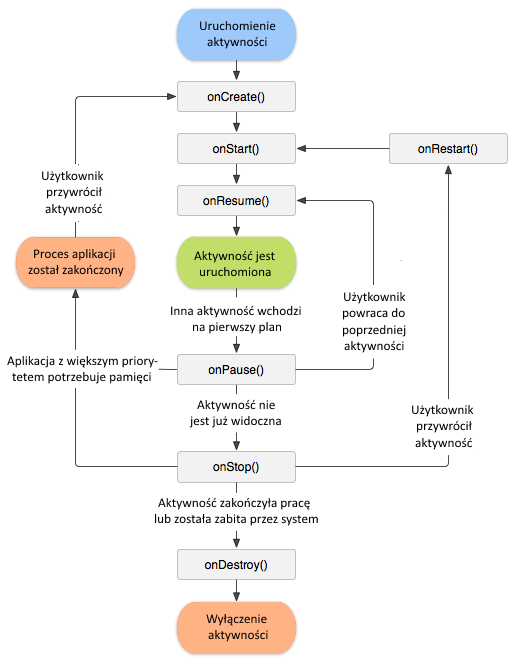
\includegraphics[scale=0.9]{imgs/activity_lifecycle_pl.png}
\caption{Cykl życia aktywności\cite{activity}}
\end{figure}

\subsection{Warstwa ograniczeń}
O Aktywności można myśleć jak o sztaludze. Jest to dopiero podstawa dla dalszej pracy. Aby namalować obraz, będzie nam potrzebne płótno. Analogicznie, aby wyświetlić coś na ekranie, będzie nam do tego potrzebna warstwa. Jest to podstawowy element interfejsu użytkownika, na którym możemy budować kolejne komponenty lub bardziej skomplikowane struktury.\par\textbf{Warstwa ograniczeń (ang. contraint layout)} to specjalna warstwa, która pozwala na pozycjonowanie komponentów oraz określenie ich wymiarów w bardzo elastyczny sposób. Dokonuje się tego za pomocą \textbf{Ograniczeń (ang. constraints)}.\par Są one relacją między komponentami. Informują o tym gdzie i w jakiej odległości leżą od siebie elementy widoku. Dzięki nim można budować interfejs na kilka sposobów. Rozmiar możemy ustawić poprzez rozciąganie lub zwężanie w dowolnych kierunkach komponentu. Wówczas mówi się, że ten element ma ustalony (ang. fixed) rozmiar. Alternatywą dla określenia wymiarów komponentu jest ustawienie, aby ograniczył się on do rozmiaru jaki zajmuje jego zawartość (ang. wrap-content). Jeśli chcemy ustalić szerokość lub wysokość, można tego dokonać za pomocą jednej z opcji: dopasuj do rodzica (ang. match-parent) lub dopasuj do ograniczeń (ang. match-constraint). Dopasowanie do rodzica spowoduje wpasowanie komponentu wertykalnie lub horyzontalnie do zewnętrznych krawędzi rodzica. Dopasowanie do ograniczeń ustali rozmiar elementu na podstawie określonych dla niego ograniczeń horyzontalnych lub wertykalnych. Jednakże należy mieć na uwadze, że bazowa klasa komponentu może nie być przystosowana do zmiany rozmiarów (np. nie posiada algorytmu skalującego domyślnej grafiki). Pozycję kolejnych elementów możemy uzależniać od pozycji już umieszczonych widoków.\par \textbf{Pozycjonowanie relatywne (ang. relative positioning)} jest najprostszym sposobem pozycjonowania. Kolejny element interfejsu użytkownika ustawiany jest wybraną krawędzią do wybranej krawędzi rodzica. 
\begin{figure}[H]
\centering
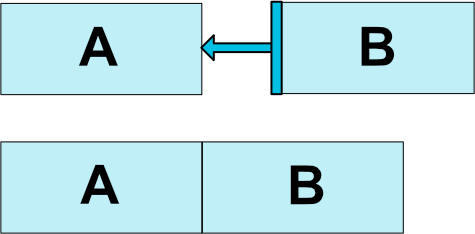
\includegraphics[scale=0.7]{imgs/relative-positioning.png}
\caption{Przykład relatywnego pozycjonowania\cite{constraintlayout}}
\end{figure} Można rozszerzyć ten mechanizm o dodatkowe marginesy. Wówczas możemy wprowadzić atrybut z wartością liczbową mówiącą o tym o ile od siebie mają być oddalone ustalone wcześniej krawędzie. \cite{constraintlayout}
\subsubsection{Elementu graficzne interfejsu}
Na utworzonej wcześniej warstie ograniczeń możemy umieszczać wybrane przez nas komponenty interfejsu graficznego. Dla każdego z komponentów ustalamy ich rozmiar oraz położenie na warstwie ograniczeń.
\paragraph{Etykieta (ang. Text View)}\mbox{}\\
Wyświetla na danym obszarze zwyły tekst. Służy głównie do przekazywania informacji. Brak interakcji z użytkownikiem.\cite{textview}
\paragraph{Przycisk (ang. Button)}\mbox{}\\
Najprostszy interaktywny element, użytkownik może w niego kliknąć co spowoduje wywołanie metody \textit{onClick()} w obiekcie Przycisku. \cite{button}
\paragraph{Przycisk wyboru (ang. Check Box)}\mbox{}\\
Ma bardzo podobne działanie do przycisku, jednakże różni się od niego tym, że posiada stan \textit{prawdy} lub \textit{fałszu}. Akcję po zmianie stanu przycisku wyboru można przeprowadzić poprzez nadpisanie metody \textit{onCheckChanged()}.
\paragraph{Pole tekstowe (ang. Edit Text)}\mbox{}\\
Kolejny prosty interaktywny element, użytkownik po kliknięciu w to pole może wprowadzić jakąś wartość. Może to być wartość liczbowa, słowna lub inna ustalona przez programistę. Służy głównie do uzyskiwania danych od użytkownika. Istnieje opcja ustawienia reagenta na zmiany wartości tego pola, jest to obiekt klasy Obserwatora Tekstu (ang. Text Watcher).\cite{edittext}
\paragraph{Lista rozwijana (ang. Spinner) i Widok listy rozszerzanej (ang. Expandable List View)}\mbox{}\\
Wyświetla opcje w postaci listy. Dla tych kontrolek niezbędne jest stworzenie dwóch dodatkowych obiektów. Adaptera, czyli obiektu zawierającego dane do wyświetlenia w odpowiednim formacie. Reagenta na wybranie pozycji z listy (ang. On Item Click Listener) i odpowiednim nadpisaniu mu metody \textit{onItemClick(AdapterView parent, View view, int position, long id)}.\cite{adapterview}
\subsection{Singleton}
Zdarza się, że w ramach naszej aplikacji chcielibyśmy posiadać globalny obiekt zawierający zestaw pól i metod, z których chcielibyśmy korzystać. Problem w tym, że każdy nowo utworzony obiekt, ma bazowe parametry, a my chcielibyśmy obiekt, który raz zmieniony zapamiętuje swoją zmianę przy kolejnych dostępach. W takiej sytuacji tworzymy właśnie Singleton, niestety nie ma dobrego polskiego tłumaczenia. Realizuje się to poprzez utworzenie w tej klasie statycznego pola, które jest obiektem tej klasy oraz statycznej metody zwracającej właśnie to pole. Oto nasza realizacja:
\begin{lstlisting}[language=Java]
public class SettingsSingleton {
    private static SettingsSingleton ourInstance = new SettingsSingleton();
    
    private SettingsSingleton(){};
    
    public static SettingsSingleton getInstance(){
        return ourInstance;
    }
}
\end{lstlisting}
Dzięki takiemu rozwiązaniu w dowolnym miejscu w kodzie możemy dostać się do obiektu \textit{SettingsSingleton} poprzez \textit{SettingsSingleton.getInstance()}. Wszelkie modyfikacje wprowadzone w tym obiekcie będą aktualne przy każdym dostępie do tego obiektu.
\subsection{System plików}
Jako użytkownik, na urządzeniu mobilnym z systemem operacyjnym Android, mamy swobodny dostęp do systemu plików poprzez interfejs graficzny. Możemy dostać się do plików dowolnej aplikacji. Jako programista również mamy dostęp do systemu plików. Możemy utworzyć folder aplikacji w pamięci urządzenia i przechowywać w nim wszelkie niezbędne dane do jej prawidłowego funkcjonowania. Dostęp do głównego katalogu pamięci urządzenia realizuje się przy pomocy klasy \textit{File}, która reprezentuje zarówno pliki jak i katalogi (zgodnie z filozofią systemu Linux). Podajemy jej w konstruktorze ścieżkę do tego folderu, można ją uzyskać poprzez statyczną metodę w klasie Środowiska (ang. Environment) -  \textit{Environment.getExternalStorageDirectory()}. Gdy mamy uchwyt do tego katalogu możemy w nim dowolnie tworzyć nowe katalogi metodą \textit{mkdirs()} lub pliki metodą \textit{createNewFile()}.
\subsection{Wibrator}
Wibrowanie urządzenia możliwe jest przy użyciu klasy Wibrator (ang. Vibrator). Obiekt tej klasy uzyskuje się poprzez wywołanie metody klasy Kontekst (ang. Context) \textit{getSystemService(Context context)}. Jako parametr \textit{context} należy podać stałą \textit{Context.VIBRATOR\_SERVICE}. Należy pamiętać, aby wynik tej metody zrzutować na klasę Wibratora.\par Najprostszym użyciem tej klasy jest wywołanie metody \textit{vibrate(long miliseconds)}, która spowoduje, że urządzenie będzie wibrowało przez podany okres. Istnieje możliwość stworzenia bardziej skomplikowanego schematu wibracji dzięki metodzie vibrate (long[] pattern, int repeat). Paremetr \textit{pattern} to tablica, której elementy stojące na nieparzystych pozycjach są okresami wibrowania, a parzyste elementy to okresy przerwy między wibracjami. Parametr \textit{repeat} informuje o tym ile razy podana sekwencja ma zostać powtórzona. Jeśli chcemy podany schemat wykonać tylko raz, należy podać w tym parametrze wartość -1. Wibrator udostępnia możliwość odgrywania efektów dźwiękowych podczas wibracji. Jeśli wyjdziemy z aktywności, która odpowiada za wibracje, nie będą one kontynuowane.\cite{vibrator}
\subsection{Aparat}

Możliwe jest użycie wbudowanego aparatu poprzez wbudowaną systemową aplikację. Wywołuje się ją przy użyciu intencji. Atrybutem określającym rodzaj akcji jest tutaj MediaStore.ACTION\_IMAGE\_CAPTURE podany jako parametr konstruktora intencji. Po utworzeniu intencji w jej dodatkach należy umieścić ścieżkę w jakiej ma być zapisane wykonane zdjęcie. W celu uruchomienia aparatu w bieżącym kontekście wołamy metodę startActivityForResult. W parametrach tej metody umieszczamy intencję oraz kod identyfikujący te wywołanie przy powrocie. Po zakończeniu działania aparatu w funkcji onActivityResult sprawdza się kod identyfikujący uruchomioną aktywność. Jeśli kod zgadza się z tym który umieściliśmy w wywołaniu aparatu, możemy wywołać akcje które powinny się wykonać zaraz po wykonaniu zdjęcie np zaktualizowanie widoku.
